\chapter{Methodology} \label{chp:chapter2}

/section{Overview}

I will combine the methods used by Hall et al. (2008) and Krstovski (2013) to the Corpus of LDS General Conference talks. I will then compare performance to that of an TF-IDF model using some of the metrics outlined by Ge et al. (2010) along with an nDCG similarity measure. This involves comparing an LDA- based recommendation system to an off-the-shelf TF-IDF recommendation system. Both systems will be parameterized such that they provide the top 5 recommendations for each document. I will use Collapsed Gibbs Sampling to induce parameters for an LDA (topic) model, then feed this output into a k-NN algorithm (k = 5). For k-NN’s distance metric, I will use Hellinger distance. The 5 nearest neighbors will then be sorted from nearest neighbor to farthest. This is the output that will be compared to the top 5 results for each document TF-IDF system.

The dataset contains the same documents as those used by Mark Davies in his Corpus of LDS General Conference talks available at http://corpus.byu.edu/gc/. The authorship dates for these talks are ranges of either 1846-1886 or 1942-2013. They total over 1400 talks. Some were extemporaneously given while others were scripted. The intended audience is generally only either the male members of the church, female members of the church, or the entire church. The size and the extent of internationality of the audience is increasing over time. The LDS church currently has over 15 million members, with the majority outside the United States.

To measure the performance of RelRec, I performed the following key tasks.

\begin{enumerate}
	\item Use \textit{Collapsed Gibbs Sampling} to infer the parameters of an LDA model;
	\item Use the Mallet toolkit will be used to run collapsed Gibbs sampling;
	\item Use k-NN with the Hellinger distance as the distance metric for RelRec; and
	\item Use nDCG to measure similarity with a TF-IDF system catalog coverage.
\end{enumerate}

\section{Reproducibility}
In order to be able to reproduce, share, and track work performed in the process of completing this thesis, I versioned code using git. I employed the use of both cutting edge tools as well as well-established ones. The result is code that is both highly capable and easy to follow. Ultimately, I aimed to make the code highly configurable, re-runable, measurable, and shareable.

In this section, methodology will be described, starting with code management \& organization, then tools used (programming languages, CLI tools, operating systems, libraries, databases), followed by models, algorithms \& metrics, concluding with metrics. In the \ref{fig:entire_process}, the steps (or modules) of the experiment are shown.

\begin{figure}[hhhhhtb]
	\centering
		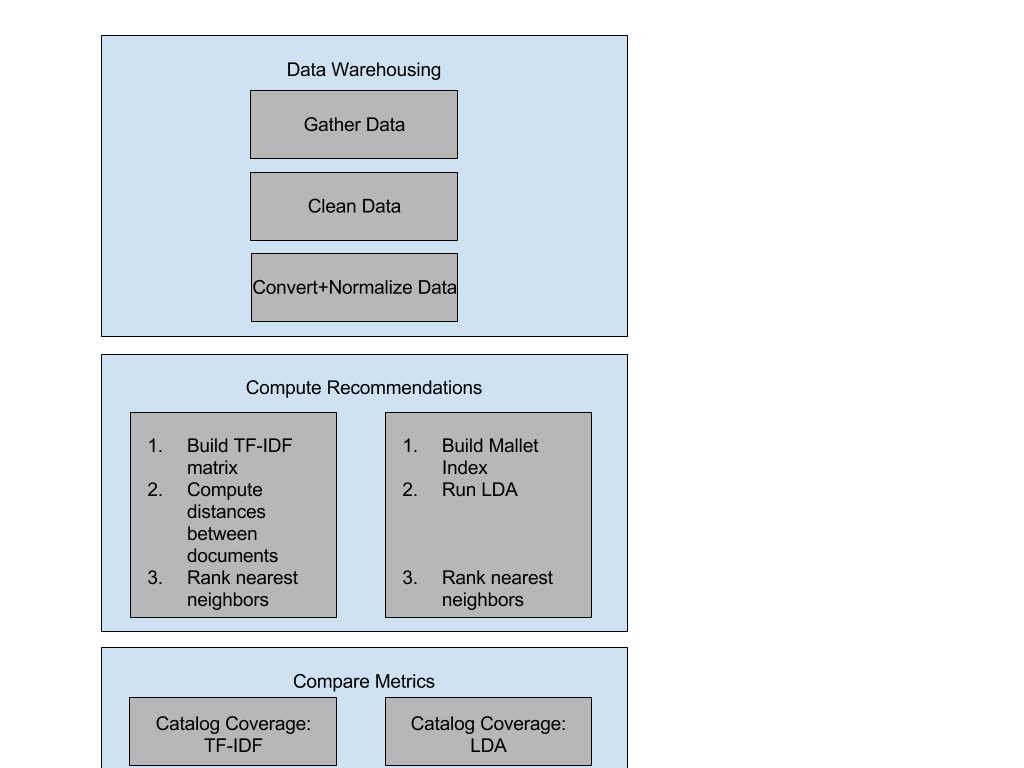
\includegraphics[width=7.5in,natwidth=810,natheight=942]{figures/entire_process.png}
		\caption[Entire Process]{
			Experiment Process\\
			The entire process for the thesis experiment outlined as `modules'. When modules are horizontally adjacent, they may be done in parallel. Note that further parallelization is possible, but not shown. Modules that are higher on the diagram are performed before lower ones.
		}
	\label{fig:entire_process}
\end{figure}

\section{Code Management + Organization}
For the experiment to be robust, it is important that it can be replicated and compared. One of the best ways to allow for this is to make the code both configurable and sharable. Thus, this section is included.

I versioned the experiment’s code in a git project along with data during the gathering process. Whenever a step completes, it outputs data which can be used as input to other modules. The code is modularized such that each docker target corresponds with a module shown previously. The docker daemon builds each target open request (as directed by make), and using docker-compose, directories are connected to the image as volumes. This allows the image to be both modular and systematic. Each docker target has a corresponding file called Dockerfile. Each Dockerfile instructs the docker daemon to obtain requisite packages, e.g. nodeJS, for the module to run the code specific to it. When the code is complete, the docker container terminates, and the next may run when Make instructs it to do so.

Viewing each docker container as a module lends to be seen as a part of the algorithm. Naturally, to each container I map an input and output folder, both located at the root of the file system. The output of multiple containers can be combined as input to subsequent ones, which was sometimes the case here. The first module’s input was actually the database graciously provided by Dr. Steven Liddle, containing pre-downloaded documents to jump-start the project.

I named each docker target logically so upon querying the docker daemon for the list of images, each image would be easy to re-run:

\begin{enumerate}
  \item obtain\_data
  \item compute\_tf\_idf\_recommendations
  \item compute\_lda\_recommendations
  \item etc.
\end{enumerate}

\subsection{Tools, Libraries, OS, Database}
I used various tools in the process of carrying for the preparation and execution of this thesis’ experiment. Table A.1 in the appendix details what they are and what they were used to do.

Core to this project was the use docker. Choosing to use docker forced me to code in all dependencies of each module either as code in the module, or as packages to be installed to each individual docker container during the docker build process. Indeed, the docker daemon builds containers by following instructions given in the files called Dockerfile. This makes each step of the experiment self-documenting. Another benefit of this is that it makes the code cloud-deployable, making it possible to easily offload work to the cloud when appropriate. Offloading to the cloud was not necessary here since I had sufficient computing resources for the project already purchased.

\subsection{Models, Algorithms \& Metrics}
Choice of algorithm \& metrics go hand-in-hand. In fact, algorithm and data can often influence each other, further influencing the selection of metrics. For example, if I were to have a gold standard or baseline of recommendation engines for the 5000+ documents used in this project, I would be able to use nDCG as a metric. Since I do not have such a baseline, such a metric cannot be used. Per xyz, I use catalog coverage, allowing the comparison of two non-baseline algorithms.

Choosing the algorithms for this project was not difficult. I selected TF-IDF+kNN and LDA+kNN as my main topic-modeling algorithms. TF-IDF is straight-forward to understand and code. LDA is more difficult to code and is actually a topic model. Luckily, open source projects exist where an algorithm is already provided, which I quickly opted to use.

Given that I had prior experience using Gibbs Sampling to generate LDA models ([TODO: Cite here.]) using the open source mallet toolkit ([TODO: cite here]), the choice to select that was logistical (optimizing to let me have time to spend on other areas of this work). EM lends itself to parallelization, but on my dataset, I knew that Gibbs Sampling would only take about 10 minutes to run, which is not an issue. The cost-benefit of changing algorithms was too high, at least when it comes to building the LDA model via parallelized algorithm. In my case, I used the mallet toolbox ([TODO: cite in introduction]) which provides the Gibbs Sampling algorithm to estimate the LDA model.

% TODO: Double check whether Jenson-Shannon was used (check prospectus).
% TODO: Add more algorithm notes here and move this table to a better location.
% TODO: 'core module' is a new term introduced here!
\begin{center}
	\begin{tabular}[pos]{| l | l | l | l | l | l |}
		\hline
		Algorithm & Variable Name & Variable Type & Input Value & Use & Reason \\ \hline

		k-NN & k & integer & 100 & Sets number of neighbors to \\ return for each document. & Using a value of 100 requires more computing, but also allows us to compare the models for up to 100 recommendations per document. \\ \hline

		Gibbs Sampling & t & integer & 250 & Sets number of topics to find & In previous research I determined that 250 was a good number for this variable. \\ \hline

		k-NN distance metric \\
		for TF-IDF model & distance & function & Cosine & Distance metric allows algorithm to measure distance between documents in the model. & Intuitive and well-known. Others functions exist for this, but are left to future work to use. \\ \hline

		k-NN distance metric \\
		for LDA model & distance & function & Jenson-Shannon & Distance metric allows algorithm to measure distance between documents in the model. & Well-known and works for vectors in the probability simplex. \\ \hline

		TF-IDF & stop words & list of word strings & none & Sets words to ignore in model. & Assigns words a value of 0 TF and 0 IDF values or removes them altogether to shrink vector space and accelerate computing (depends on actual algorithm implementation). TF-IDF is robust against high-frequency words since they automatically receive low TF and low IDF values. \\ \hline

		Preparing input LDA & stop words & list of word strings & default mallet list + handful of religious words [TODO: which words?] & Removes stopwords at indexing time (module x [TODO: name exact module here]). & LDA is not super robust against common words. \\ \hline
		normalization & to\_lower\_case & boolean & true & If true, tells algorithm to lowercase all text. & To allow all following algorithms to ignore case, the simplest way to do so was to lowercase everything before completing the data preparation core module. \\ \hline
	\end{tabular}
\end{center}

% TODO: cite instead of link?
The core of this project came down to organization, good testing (to ensure bug-free code), and study of any tools that would end up being helpful in processing. kNN is a machine learning algorithm which as input requires the value for k and a selection of a distance metric. The output of TF-IDF and LDA are both in vectors, but LDA’s vectors lay within the probability simplex. Distance metrics had to be appropriate for the space. For TF-IDF vectors, I opted to use cosine similarity; for LDA, Jensen-Shannon (\url{https://en.wikipedia.org/wiki/Jensen%E2%80%93Shannon_divergence, http://maroo.cs.umass.edu/pub/web/getpdf.php?id=1101}). % TODO: (or was it Hellinger? \url{https://www.quora.com/How-can-I-compute-the-Hellinger-distance-between-documents-based-on-topic-proportions-generated-by-Latent-Dirichlet-Allocation}).

To evaluate the recommendations provided as output from the ordered kNN results, a common metric had to be employed. I chose to measure the goodness of each set using the catalog coverage metric. % TODO: remove passive voice here.

For reproducibility, the following table shows the values, settings, and configurations selected for the algorithms.

By using the aforementioned metrics, this study aims to prove the following hypothesis
	\begin{quote}
		$H_{1}:$ \emph{RelRec} will provide better coverage than a \emph{TF-IDF} system.

		%$H_{2}:$ RelRec is more intuitive than emph recommendation systems since it has greater ability to disambiguate word sense by topic.
	\end{quote}
